\section{Theory}

\subsection{Inspiration} \label{Inspiration}
As shown in Section \ref{current_literature}, the development of the use of fractional order calculus from a purely mathematical construct to one of use in pharmacokinetics is a recent development which has in part been been influenced by the failure of traditional integer order systems to accurately describe the dynamics of certain drugs. The development of the use of fractional order dynamics is also in part related to changes in the computational processing capabilities of many researchers in recent years. Having said this however, another area which has also made significant use of fractional order calculus is control theory \cite{Fractional_order_control, FOC_Basics, control_theory_fractional_applications, fractional_control_tutorial}. Use of fractional order dynamics in control systems has allowed for greater stability within these systems. Additionally it also allows engineers greater control via a wider range of parameters for modelling physical phenomena.

It is therefore unfortunate that despite the common use of this technique in control, the way in which it is used is different than the way in which many other fields would, at least initially, wish to use it. The problem being that outside control, parameter estimation, (with respect to values such as the order and the initial conditions of the system), is a highly useful technique in the context of fractional order systems. This of course resulted in a lack of attention being given to fractional order methods of characterising systems outside control, which was one of the few areas in which the order, and other parameters are selected in advance of their use and left unchanged.

\subsection{Modelling System Dynamics} \label{Modelling_System_Dynamics}

In pharmacokinetic systems, the adsorption, distribution, metabolism, and excretion of drugs is modelled through the use of differential dynamics equations for flow of the drugs between compartments within the body. At the most basic level a compartment model of the human body can consist of a single compartment (known as the central compartment), which typically has its concentrations represented by the concentrations present in blood plasma \cite{Compartmental_modeling_in_Pharmacokinetics, One_Compartment_Open_Model}. The system shown in Figure \ref{fig:single_compartment_model} is an example of this model. 

\begin{figure}[h]

	\begin{center}
	
		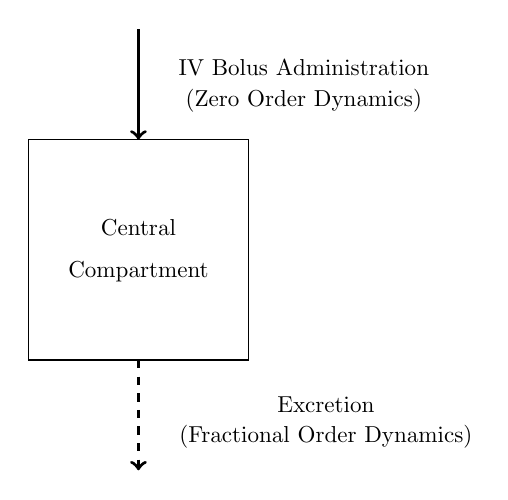
\begin{tikzpicture}[scale=1.4]
		
		% Draw Shape
		\draw[->, very thick] (0,0) -- (0, -1);
		\draw[thin] (-1,-3) rectangle (1, -1);
		\draw[->, dashed, very thick] (0,-3) -- (0, -4);
		
		% Labels
		\draw node[scale=10/12] at (1.5, -0.35) {IV Bolus Administration};
		\draw node[scale=10/12] at (1.5, -0.65) {(Zero Order Dynamics)};
		
		\draw node[scale=10/12] at (0, -1.8) {Central};
		\draw node[scale=10/12] at (0, -2.2) {Compartment};
		
		\draw node[scale=10/12] at (1.7, -3.4) {Excretion};
		\draw node[scale=10/12] at (1.7, -3.7) {(Fractional Order Dynamics)};
		
		\end{tikzpicture}
	
	\end{center}
	\caption{Example of a single compartment model of the human body with fractional order dynamics}
    \label{fig:single_compartment_model}
    
\end{figure}

Of course this model is very simple and does not fully describe the infinite complexity that could be gone into with respect to pharmacokinetics in the body. Other models which are typically used in the modelling of drugs include 3 and 7 compartment models, which take into account various different types of tissue in the body with similar dynamical properties. An example of a 3 compartment model involving fractional order pharmacokinetics is shown in Figure \ref{fig:three_compartment_model}.

\begin{figure}[h]

	\begin{center}
	
		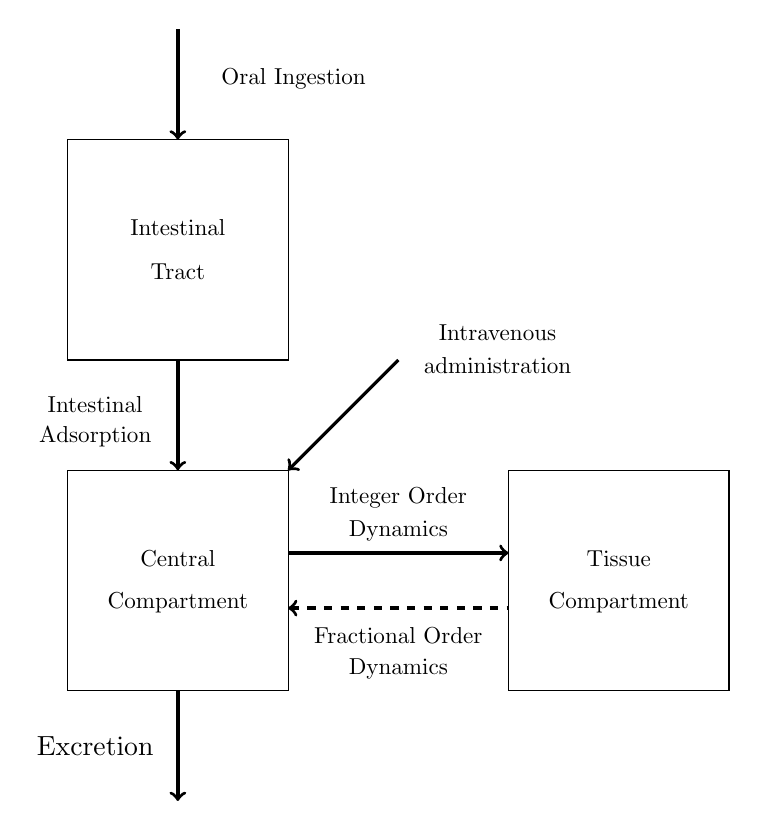
\begin{tikzpicture}[scale=1.4]
		
		% Draw Shape
		\draw[->, very thick] (0,0) -- (0, -1);
		\draw[thin] (-1,-3) rectangle (1, -1);
		\draw[->, very thick] (0,-3) -- (0, -4);
		\draw[thin] (-1,-4) rectangle (1, -6);
		\draw[<-, dashed, very thick] (1, -5.25) -- (3, -5.25);
		\draw[->, very thick] (2, -3) -- (1, -4);
		\draw[->, very thick] (1, -4.75) -- (3, -4.75);
		\draw[->, very thick] (0, -6) -- (0, -7);
		\draw[thin] (3,-4) rectangle (5, -6);
		
		% Labels
		\draw node[scale=10/12] at (0, -1.8) {Intestinal};
		\draw node[scale=10/12] at (0, -2.2) {Tract};
		
		\draw node[scale=10/12] at (0, -4.8) {Central};
		\draw node[scale=10/12] at (0, -5.2) {Compartment};
		
		\draw node[scale=10/12] at (4, -4.8) {Tissue};
		\draw node[scale=10/12] at (4, -5.2) {Compartment};
		
		\draw node[scale=10/12] at (1.05, -0.45) {Oral Ingestion};
		
		\draw node[scale=10/12] at (-0.75, -3.4) {Intestinal};
		\draw node[scale=10/12] at (-0.75, -3.7) {Adsorption};
		
		\draw node[scale=10/12] at (2.9, -2.75) {Intravenous};
		\draw node[scale=10/12] at (2.9, -3.05) {administration};
		
		\draw node[scale=10/12] at (2, -4.25) {Integer Order};
		\draw node[scale=10/12] at (2, -4.55) {Dynamics};
		
		\draw node[scale=10/12] at (2, -5.5) {Fractional Order};
		\draw node[scale=10/12] at (2, -5.8) {Dynamics};
		
		\draw node at (-0.75, -6.5) {Excretion};
		
		\end{tikzpicture}
	
	\end{center}
	\caption{Example of a three compartment model of the human body with fractional order dynamics for the drug Amiodarone \cite{kuhlkamp1999effect}}
    \label{fig:three_compartment_model}
    
\end{figure}

One issue that is issue present in these models however, is that with more than one compartment, modelling the dynamics quickly becomes significantly more complex, particularly if one or more of the compartments has fractional order dynamics governing the flow in or out of it. This is in part because maintaining the conservation of mass of the drug in each compartment becomes highly complex when estimating the order of each dynamics equation, along with other parameters due to the interdependence between each equation. It is for this reason that this project was specifically focussed on modelling the excretion from a single compartment system, as shown in Figure \ref{fig:single_compartment_model}. 

In addition to the modelling of the system via compartmental methods, it is important to note that the dynamical equations which are used to describe the flow of the drug, in the case of the model in \ref{fig:single_compartment_model} out of the body, can be considered to be either fractional, first, or zero order equations. Given the wide variety of different equations which may be used to describe these phenomena, and that they may be of varying order, this paper therefore uses a simple exponential equation to test the methods when programmed and leaves the dynamical equation open to change by the end user.

\subsection{Fractional Order Derivatives and Pharmacokinetics}\label{fod_and_pharmacokinetics}

Fractional Order Differential Equations are a class of differential equation which there has been interest in nearly as long as Integer Order Differential Equations, with it first being mentioned in a letter between Leibniz and L'Hospital in 1695 \cite{the_fractional_calculus}. Since then the earliest systematic studies of the idea began in the early 19th century. 

In modern terms, the primary forms of the fractional order derivative in the context of pharmacokinetics are the Caputo, Riemann-Liouville and the Gr\"{u}nwald-Letnikov derivatives, each of which is slightly different in terms of it's definition. One such difference it that when using the Caputo definition for example, taking the derivative of a constant is in fact 0, compared to the Riemann-Liouville definition for which this is not true. These differences are possible as each definition is applicable to a different situation. Despite these differences however, one element all of these definitions have in common is that they collapse back into the standard definition for a derivative when the order is an integer. 

The reasoning for their use with respect to the field of pharmacokinetics, as partially explained in Section \ref{Modelling_System_Dynamics}, is tied to the ability of fractional order derivatives to take into account an infinite history of a system, not just the local history at a particular point. Another reason which should be noted as significantly important is that the systems in question are fractional order in nature, i.e. they exhibit non-linear fractional order behaviour when they are observed.

Despite the large volume of material in this subject area for the purposes of this project, the primary focus shall be the implementation of the Gr\"{u}nwald-Letnikov (GL) derivative. The reasoning behind this is primarily related to the ability to easily discretise the GL derivative. This ability means that this method can be used to approximate fractional order differential equations.

\subsection{Gr\"{u}nwald-Letnikov Derivatives} \label{gl_derivatives}

Gr\"{u}nwald-Letnikov (GL) derivatives are fundamentally an extension of the most basic numerical method of obtaining first order derivatives, Euler's method, such that the order being solved can be a non-integer value \cite{the_fractional_calculus, euler1794institutiones}. Given some function $\gls{general_function}$, with a derivative of $\gls{first_order}$, dependent variable $\gls{general_dependent_variable}$, and a step of $\gls{time_step}$, Euler's method is given by the equation,
\begin{equation}\label{eulers_method}
	f^{\prime}(x) = \lim_{h \to 0} \frac{f(x)-f(x-h)}{h} \approx \frac{f(x)-f(x-h)}{h},
\end{equation} 
provided that $\gls{time_step} > 0$ and is sufficiently small. It can be noted at this point that assuming that $\gls{general_function}$ is continuously differentiable, Equation \ref{eulers_method} is simply a first order approximation using Taylors theorem. 

Therefore, using Equation \ref{eulers_method}, a second order derivative of a function, as given by $\gls{second_order}$ can also be obtained through iteratively applying this method. Doing so gives rise to the equation,
\begin{equation}\label{second_order}
	f^{\prime\prime}(x)= \lim_{h \to 0} \frac{f^{\prime}(x)-f^{\prime}(x-h)}{h} \approx \frac{f^{\prime}(x)-f^{\prime}(x-h)}{h},
\end{equation}
which of course can be expanded out and simplified such that no intermediate step of calculating the first order derivative is required,
\begin{equation}\label{second_order_expanded}
	f^{\prime\prime}(x) = \lim_{h \to 0} \left\{\frac{\left(\frac{f(x)-f(x-h)}{h}\right)-\left(\frac{f(x-h)-f(x-2h)}{h}\right)}{h}\right\},
\end{equation}
\begin{equation}\label{second_order_simplified}
	f^{\prime\prime}(x) = \lim_{h \to 0} \left\{\frac{1}{h^{2}}\left\{f(x)-2f(x-h)+f(x-2h)\right\}\right\},
\end{equation}
doing this again for the third order derivative $\gls{third_order}$, gives rise to this equation,
\begin{equation}\label{third_order}
	f^{\prime\prime\prime}(x)= \lim_{h \to 0} \frac{f^{\prime\prime}(x)-f^{\prime\prime}(x-h)}{h} \approx \frac{f^{\prime\prime}(x)-f^{\prime\prime}(x-h)}{h},
\end{equation}
simplified, 
\begin{equation}\label{third_order_simplified}
	f^{\prime\prime\prime}(x) = \lim_{h \to 0} \left\{\frac{1}{h^{2}}\left\{f(x)-3f(x-h)+3f(x-2h)-f(x-3h)\right\}\right\},
\end{equation}
which allows a pattern that is forming to be observed. The binomial expansion that is present in the simplified forms of the equations Equation \ref{second_order_simplified} and Equation \ref{third_order_simplified} mean that these can therefore be defined in terms of a general equation that can be used for obtaining any $\gls{n}$ order derivative $\gls{general_order_derivative}$ of a given function $\gls{general_function}$,
\begin{equation}\label{third_order_generified}
	f^{\prime\prime\prime}(x) = \lim_{h \to 0} \left\{\frac{1}{h^{3}}\sum_{j=0}^{3} (-1)^{j} {3 \choose j} f(x-jh)\right\},
\end{equation}
\begin{equation}\label{general_order}
	f^{(n)}(x) = \lim_{h \to 0} \left\{\frac{1}{h^{n}}\sum_{j=0}^{n} (-1)^{j} {n \choose j} f(x-jh)\right\}.
\end{equation}

Equation \ref{general_order} therefore is the general equation for obtaining a derivative of any order. The final step which results in the GL derivative is to extend the binomial coefficient operator such that instead of using the factorial in the calculation, the $\Gamma$ function is used in its place. This means using the identity $\Gamma(\Omega+1) = \Omega!$, for any real number $\Omega$. Doing this means that the binomial operator is replaced with,
\begin{equation}\label{extended_binomial}
	{\alpha \choose j} = \frac{\Gamma(\alpha + 1)}{j!\Gamma(\alpha-j+1)}.
\end{equation}

Upon replacement, the only remaining element left to change is that the value of $n$ as the upper limit in the sum must be changed so it is still an integer value. To do this, the floor of the current point $x$, divided by the time step (i.e. how many previous points in history there are), must be used. This means that the overall GL derivative for an order of $\gls{fractional_order}$ is given by,
\begin{equation}\label{gl_order}
	^{gl}D^{\alpha}_{x}f(x) = \lim_{h \to 0} \left\{\frac{1}{h^{\alpha}}\sum_{j=0}^{\lfloor\frac{x}{h}\rfloor} (-1)^{j} {\alpha \choose j} f(x-jh)\right\}.
\end{equation}

\subsection{Discretisation And Computability}

Based on the equations for the GL derivative highlighted in Section \ref{gl_derivatives}, the first step to allow the computability of the function is to define the extended form of the binomial coefficient operator in such a way as to allow a computer with a finite number of bits to be able to calculate it. To do this, the following equation may be used instead of Equation \ref{extended_binomial}, as the use of Gamma function means in most cases it use is not practical. The equation,
\begin{equation}\label{computable_extended_binomial}
	{\alpha \choose j} = \prod_{i=0}^{j-1}\frac{\alpha-1}{i+1}.
\end{equation}
can therefore be substituted in its place \cite{Fractional_calculus_in_pharmacokinetics}. 

Having said this, to have the ability to compute the GL derivative, it must be discretised. As the GL method is based on a numerical method already, this is trivial. Equation \ref{gl_order} needs only be moved from the continuous domain of $x$ to a discrete domain defined by a step of $\gls{time_step}$ in order to become discretised, with an appropriately small value of $h$ allowing near approximation of the original function. To index each time step, an index $\gls{time_step_index}$ is used, such that $k=\frac{x}{h}$ where $x$ is the current point in the dependent variable and the discrete fractional order differential equation is given by $^{gl}D^{\alpha}_{x}f(x) = z(f)$, meaning the new equation shall be, 
\begin{equation}\label{gl_semi_ddiscretised_order}
	^{gl}D^{\alpha}_{x}f(x) \approx \frac{1}{h^{\alpha}}\sum_{j=0}^{\lfloor\frac{kh}{h}\rfloor+1} (-1)^{j} {\alpha \choose j} f(kh - jh + h) = z(f(kh)),
\end{equation}
\begin{equation}\label{gl_discretised_order}
	 h^{\alpha}z(f_{k}) = {\alpha \choose 0} f_{k+1} + \sum_{j=0}^{k+1} (-1)^{j} {\alpha \choose j} f_{k - j + 1}
\end{equation}

The final step to allow for this to be used in running a simulation is now to rearrange the equation such that the solution to the fractional order differential equation is the subject. To do this, first, since ${\alpha \choose 0}$ is always 1 it can be removed, next Equation \ref{gl_discretised_order} can be rearranged to give,
\begin{equation}\label{gl_solution}
	f_{k+1} = h^{\alpha}z(f_{k}) - \sum_{j=0}^{k+1} (-1)^{j} {\alpha \choose j} f_{k - j + 1}.
\end{equation}

This form of the GL Method can now be used to solve fractional order pharmacokinetics equations, where $f = x$ (i.e. the concentration), $x = t$ (i.e. the time) and $z = \phantom{}^{gl}D^{\alpha}_{x}x(t)$ (i.e. a fractional order dynamics equation) in pharmacokinetics. This of course means the equation is therefore written as,
\begin{equation}\label{gl_pk_solution}
	x_{k+1} = h^{\alpha}\phantom{ }^{gl}D^{\alpha}_{x}x(t_k) - \sum_{j=0}^{k+1} (-1)^{j} {\alpha \choose j} x_{k - j + 1},
\end{equation}
with a bound for the order, $\alpha$, of $0 < \alpha \leq 1$, as to have an alpha greater than one would make no physical sense as it could cause negative concentrations \cite{Fractional_calculus_in_pharmacokinetics}.

\subsection{Estimation}

In order to be able to fit parameters to allow for the estimation of values, the cost function for the optimisation problem must be formed. In terms of this project, initially a version of the least-squares method was used to get an idea how good estimating the parameter values may be given a perfect model with no error or noise, and a non-sparse dataset which has moderate to high levels of measurement noise. To do this, the cost function, Equation \ref{cost_function_one} was implemented, where the sum squared error $\epsilon$ was calculated across $k$ data points $y_{n}$ and the estimations for a given set of model parameters, $x_{n}$, where $n$ is the index in both cases. This is of course subject to the model $F_{t}(x_{0} \dots x_{t}, \alpha, \theta)$, where the finite history, $\alpha$ and $x_{0}$ are used to calculate the solution to the fractional differential equation as the order and initial condition respectively and $\theta$ represents any other parameters in the system, thus giving,
\begin{subequations}
	\begin{align}\label{cost_function_one}
		\operatorname{Minimise} \epsilon(x_{0} \dots x_{t}, \theta) &= \sum_{t=0}^{k} (y_{t}-x_{t})^{2},
	\intertext{subject to:}
		x_{t} &= F_{t}(x_{0} \dots x_{t-1}, \alpha, \theta), \text{ for } t = 1 \dots k,\\
		x_{t} &\geq 0,\\
		\alpha &> 0,\\
		\theta &> 0.
	\end{align}
\end{subequations}

This method in practice works very well, however it makes an assumption that the model that is used is perfect, and that the dataset can exactly fit this model. To take into account estimation noise $w_{t}$ which may be present in the system, the cost function may be updated,
\begin{subequations}
	\begin{align}\label{cost_function_two}
		\operatorname{Minimise} \epsilon(x_{0} \dots x_{t}, \theta) &= \sum_{t=0}^{k} (y_{t}-x_{t})^{2} + w_{t}^{2},
	\intertext{subject to:}
		x_{t} &= F_{t}(x_{0} \dots x_{t-1}, \alpha, \theta) + w_{t}, \text{ for } t = 1 \dots k,\\
		x_{t} &\geq 0,\\
		\alpha &> 0,\\
		\theta &> 0.
	\end{align}
\end{subequations}

Passing these cost functions into an optimisation algorithm such as the L-BFGS-B algorithm \cite{L_BFGS_B_Method} or a particle swarm algorithm \cite{wang2018particle} will allow for an optimum solution to be found easily. The only important element regarding the optimisation algorithm to take into account is the ability to place box constraints on the parameters being optimised such as to avoid clearly illogical values such as negative concentrations.

Once optimum values have been achieved, the process can be ran a significant number of times (simulating multiple experimental datasets with different additive noise), to perform a Markov Chain Monte Carlo simulation to allow the production of probability distribution functions for the estimated parameters. This is done to check the system for its ability to withstand measurement noise and to see how estimations vary with different levels of noise.

This concept of characterising noise and response to noise and variation in the estimated parameters therefore leads onto utilising a Bayesian statistical methodology to allow prior knowledge of the noise and characteristics associated with each parameter to be taken into account. For the value of $\alpha$ when estimating it for a whole dataset, it will likely be best to use a beta distribution for the prior, as this allow for values near the extremes to be less likely (as these values would suggest that the dynamics are not in fact fractional but is likely closer to integer order dynamics). Additionally, the distribution of the initial condition $x_{0}$ is considered to be normally distributed around a mean of a high value as values close to zero are unlikely for this as the concentration when excreting must always go from high to low. The sources of noise in this system are all presumed for now to be normally distributed, however experimental data and information regarding the measurement tools will allow this to change once more prior information is available. 

Using these priors, the cost function highlighted in Equation \ref{cost_function_two} can be modified to obtain a posterior distribution for each parameter which should have an improved credibility interval. The updated cost function also takes into account estimation noise $w_{t}^{\alpha}$, $w_{t}^{\theta}$, and $w_{t}$ as well as measurement noise $v_{t}$ which is present in the experimental dataset. 

The three distributions which are to be used in this updated cost function are the normal, beta and exponential distributions. Putting these into log form for the cost function is a simple process. For the normal distribution, the probability density function is defined by the following equation where $\mu$ is the mean, $\sigma$ is the standard deviation, and x is the variable that is normally distributed, 

\begin{equation}\label{pdf_normal}
	p_{x}(x) = \frac{1}{\sqrt{2\pi}\sigma} \exp{(-\frac{1}{2}(\frac{x-\mu}{\sigma})^{2})},
\end{equation}

As we have the assumption any noise present in the system is unbiased the mean can be assumed to be 0. This gives rise to a new equation which the log is taken of, before one of the rules of logarithms is applied to separate the product term in the equation,
\begin{equation}\label{unbiased_log_pdf_normal}
	-\ln(p_{x}(x)) = \log{\frac{1}{\sqrt{2\pi}\sigma}} + \log{\exp{(-(\frac{x}{2\sigma})^{2})}},
\end{equation}
As the first term in the sum is a constant it can be disregarded, leaving the second term which can be simplified again as the log and exponent cancel out. This means the prior for the normally distributed parameters in the system is able to now be given by,
\begin{equation}\label{unbiased_log_pdf_normal}
	-\ln(p_{x}(x)) = (\frac{x^{2}}{2\sigma}).
\end{equation}
In addition to this, the exponential distribution is used. This is again, simple to write logarithmically, with the original probability density function being,
\begin{equation}\label{unbiased_log_pdf_normal}
	p_{x}(x) = \gamma\exp(-\gamma x),
\end{equation}
where the parameter $\gamma$ is a parameter set by the user. To write this in terms of a log, the rule of logs regarding product terms is again used to remove a $\gamma$ term as a constant, before again the log cancels out with the exponential, leaving,
\begin{equation}\label{unbiased_log_pdf_normal}
	\ln{p_{x}(x)} = -\gamma x.
\end{equation}
The final distribution used in this cost function shall be the beta distribution, which is defined by two parameters, a and b. The probability density function for this distribution is simple to understand, and as such again is simple to write in terms of a logarithmic formulation. The function is,
\begin{equation}\label{unbiased_log_pdf_normal}
	p_{x}(x) = \frac{x^{a - 1}1-x^{b - 1}}{\frac{\Gamma(a) \Gamma(b)}{\Gamma(a+b)}}.
\end{equation}

Once again, the first step in converting this to a logarithm is to use one of the rules of logs to separate the numerator and denominator from each other. This allows the denominator to be removed as a constant. Following this, again using the rule of logs regarding products, the numerator can be separated out into two different terms being summed,
\begin{equation}\label{unbiased_log_pdf_normal}
	\ln{p_{x}(x)} = \ln{x^{a-1}} + \ln{(1-x)^{b-1}}.
\end{equation}

The final step is then to use the log power rule to remove the power terms, giving the following,
\begin{equation}\label{unbiased_log_pdf_normal}
	\ln{p_{x}(x)} = (a-1)\ln{x} + (b-1)\ln{1-x}.
\end{equation}

Using these distributions and substituting in estimated parameters instead of x, the cost function is therefore,
\begin{subequations}
	\begin{align}\label{cost_function_three}
		\operatorname*{Minimise}_{\alpha, \theta, w_{t}, w_{t}^{\alpha}, w_{t}^{\theta}, v_{t}} &\sum_{t=0}^{k} (\frac{w_{t}}{\sigma_{w}}^{2}+\frac{w_{t}^{\alpha}}{\sigma_{w}^{\alpha}}^{2}+\frac{w_{t}^{\theta}}{\sigma_{w}^{\theta}}^{2}+\frac{v_{t}}{\sigma_{v}}^{2}) \notag\\
		&- ((a-1)\ln(\alpha)+(b-1)\ln(1-\alpha)) \notag\\
		&- (\gamma x_0),
	\intertext{subject to:}
		x_{t} &= F_{t}(x_{0} \dots x_{t-1}, \alpha, \theta) + w_{t}, \text{ for } t = 1 \dots k,\\
			\alpha_{t+1} &= \alpha_{t} +  w_{t}^{\alpha},\\
			\theta &= \theta + w_{t}^{\theta},\\
			y_{t} &= x_{t} + v_{t},\\
			x_{t} &\geq 0,\\
			\alpha &> 0,\\.
	\end{align}
\end{subequations}

These methods of course require a full dataset of nearly continuous data to work, however a small change in the method of performing the minimisation can correct for this, with the moving horizon estimate one option that may be used for a continuous stream of data for which is it not possible to have a full history stored without memory issue. Another option may be to simply perform the minimisation over the data points which are present in the experimental data, i.e. instead of a sum over all points from 0 to the maximum time at steps of size $h$, simply index the times which measurements were taken and compare these to the estimated values. The use of the a priori methodology should also help here, with details of the distribution for each parameter helping to guide the maximum likelihood method which has been used.
